% \iffalse
\let\negmedspace\undefined
\let\negthickspace\undefined
\documentclass[journal,12pt,twocolumn]{IEEEtran}
\usepackage{cite}
\usepackage{amsmath,amssymb,amsfonts,amsthm}
\usepackage{algorithmic}
\usepackage{graphicx}
\usepackage{textcomp}
\usepackage{xcolor}
\usepackage{txfonts}
\usepackage{listings}
\usepackage{enumitem}
\usepackage{mathtools}
\usepackage{gensymb}
\usepackage{comment}
\usepackage[breaklinks=true]{hyperref}
\usepackage{tkz-euclide} 
\usepackage{listings}
\usepackage{gvv}                                        
\def\inputGnumericTable{}                                 
\usepackage[latin1]{inputenc}                                
\usepackage{color}                                            
\usepackage{array}                                            
\usepackage{longtable}                                       
\usepackage{calc}                                             
\usepackage{multirow}                                         
\usepackage{hhline}                                           
\usepackage{ifthen}                                           
\usepackage{lscape}

\newtheorem{theorem}{Theorem}[section]
\newtheorem{problem}{Problem}
\newtheorem{proposition}{Proposition}[section]
\newtheorem{lemma}{Lemma}[section]
\newtheorem{corollary}[theorem]{Corollary}
\newtheorem{example}{Example}[section]
\newtheorem{definition}[problem]{Definition}
\newcommand{\BEQA}{\begin{eqnarray}}
\newcommand{\EEQA}{\end{eqnarray}}
\newcommand{\define}{\stackrel{\triangle}{=}}
\theoremstyle{remark}
\newtheorem{rem}{Remark}
\begin{document}

\bibliographystyle{IEEEtran}
\vspace{3cm}

\title{NCERT 11.9.2.3}
\author{EE23BTECH11043 - BHUVANESH SUNIL NEHETE$^{*}$% <-this % stops a space
}
\maketitle
\newpage
\bigskip

\renewcommand{\thefigure}{\theenumi}
\renewcommand{\thetable}{\theenumi}

\bibliographystyle{IEEEtran}

\section*{Question}

In an A.P. the first term is 2 and the sum of the first five terms is one-fourth of the next five terms. Show that 20\textsuperscript{th} term is $-112$

\section*{Solution}

\[T_1 + T_2 + T_3 + T_4 + T_5 = \frac{1}{4} [T_6 + T_7 + T_8 + T_9 + T_{10}]\]
Let the first term \(a\) and the common difference \(d\):
\[[a + (a + d) + (a + 2d) + (a + 3d) + (a + 4d)] =\] 
\[\frac{1}{4} [(a + 5d) + (a + 6d) + (a + 7d) + (a + 8d) + (a + 9d)]\]
Simplifying:
\[(5a + 10d) = \frac{1}{4}(5a + 35d)\]
\[20a + 40d = 5a + 35d\]
\[15a + 5d = 0\]
\[3a + d = 0 \implies d = -3a \implies d = -6 \quad (\text{given } a = 2)\]
\[T_{20} = a + 19d = 2 + 19(-6) = -112\]

\[a=2\quad and\quad d=-6\]
\[t_{n}=a+(n-1)d\]
\[\implies t_{n}=2+(n-1)(-6)\]
\[\implies t_{n}=8-6n\]
The Z-transform of a sequence $t_n$ is given by:

\[ T(z) = \sum_{n=0}^{\infty} t_n z^{-n} \]

For the sequence $t_n = 8 - 6n$ when $n > 0$, we can write:

\[ T(z) = \sum_{n=1}^{\infty} (8 - 6n)z^{-n} \]

Now, let's manipulate this expression. We can split it into two parts:

\[ T(z) = \sum_{n=1}^{\infty} 8z^{-n} - \sum_{n=1}^{\infty} 6nz^{-n} \]

\begin{enumerate}
    \item \[\sum_{n=1}^{\infty} 8z^{-n}=8\sum_{n=1}^{\infty} z^{-n}\]
    \[\hspace{3.9cm}=8(z^{-1}+z^{-2}+z^{-3}+\dots)\]
    \[\hspace{1.4cm}=\frac{8z^{-1}}{1-z^{-1}}\]

    \item \[\sum_{n=1}^{\infty} 6nz^{-n}=6\sum_{n=1}^{\infty}nz^{-n}\]
    \[\hspace{3.9cm}=6(1\cdot z^{-1} + 2\cdot z^{-2} + 3\cdot z^{-3} + \dots)\]
    This is AGP.
    \[S=1\cdot z^{-1}+2\cdot z^{-2}+3\cdot z^{-3}+\dots\]
    \[-\hspace{0.5cm}z^{-1}S=\hspace{1.5cm}1\cdot z^{-2}+2\cdot z^{-3}+3\cdot z^{-4}+\dots\]
    \hrulefill
    \[(1-z^{-1}S)=z^{-1}+z^{-2}+z^{-3}+z^{-4}+\dots\]
    \[(1-z^{-1})S=\frac{z^{-1}}{1-z^{-1}}\]
    \[S=\frac{z^{-1}}{(1-z^{-1})^{2}}\]
    \[\implies \sum_{n=1}^{\infty}6nz^{-n}=\frac{6z^{-1}}{(1-z^{-1})^{2}}\]
\end{enumerate}
\vspace{1cm}
\[T(z)=\frac{8z^{-1}}{1-z^{-1}}+\frac{6z^{-1}}{(1-z^{-1})^{2}}\]

\newpage

\begin{figure}
    \centering
    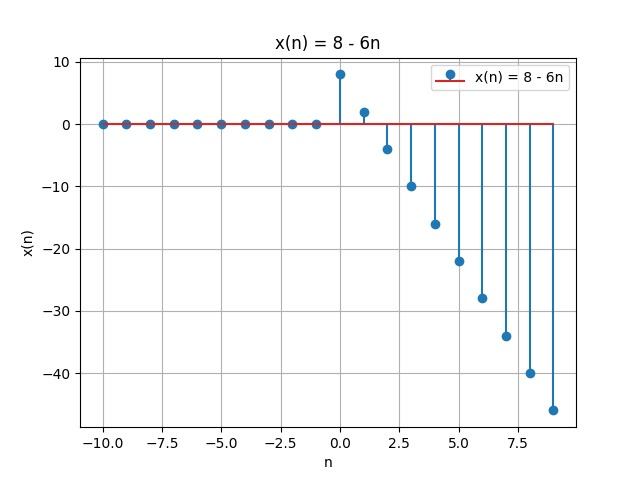
\includegraphics[width=1\linewidth]{Figure_1.png}
    \[Fig. 1\hspace{2mm}x(n) = 8 - 6n\]
\end{figure}

Given that \( n > 0 \), let's analyze the ROC for the Z-transform of the sequence \( x[n] = 8 - 6n \):

\[X(z) = \sum_{n=1}^{\infty} (8 - 6n) \cdot z^{-n}\]

For convergence, the series 
\vspace{2mm}
\[\sum_{n=1}^{\infty} (8 - 6n) \cdot |z|^{-n}\]

\vspace{2mm}
must converge. This implies that \( |z| \) should be greater than the magnitude of the terms \( (8 - 6n) \). The terms \( (8 - 6n) \) decrease in magnitude as \( n \) increases, so the ROC is the set of complex numbers \( z \) such that \( |z| \) is greater than the magnitude of the terms for all \( n \).
\vspace{2mm}

In this case, the ROC is the region outside the circle with radius equal to the magnitude of the first term \( |8| \) in the series, i.e.; outside the circle \( |z| > 8 \).
\vspace{2mm}

So, the Region of Convergence (ROC) for the Z-transform of the sequence \( x[n] = 8 - 6n \) with \( n > 0 \) is the exterior of the circle \( |z| > 8 \).

\end{document}
